\subsection{题目描述}
\noindent
Solve the time-dependent Schrödinger equation using both the Crank–Nicolson scheme and a stable explicit scheme. Consider the one-dimensional case and test it by applying it to the problem of a square well with a Gaussian initial state coming in from the left.

\noindent
Hint: The Gaussian initial state could be expressed as:
\[
    \Psi(x, 0) = \sqrt{\frac{1}{\pi}} \exp\left[ i k_0 x - \frac{(x - \xi_0)^2}{2} \right].
\]


\subsection{程序描述}

\subsection{伪代码}
Powered by \href{https://chatgpt.com/g/g-xJJAA2awf-latex-pseudocode-generator}{\LaTeX \ pseudocode generator}


\subsection{结果示例}
\begin{figure}[H]
    \centering
    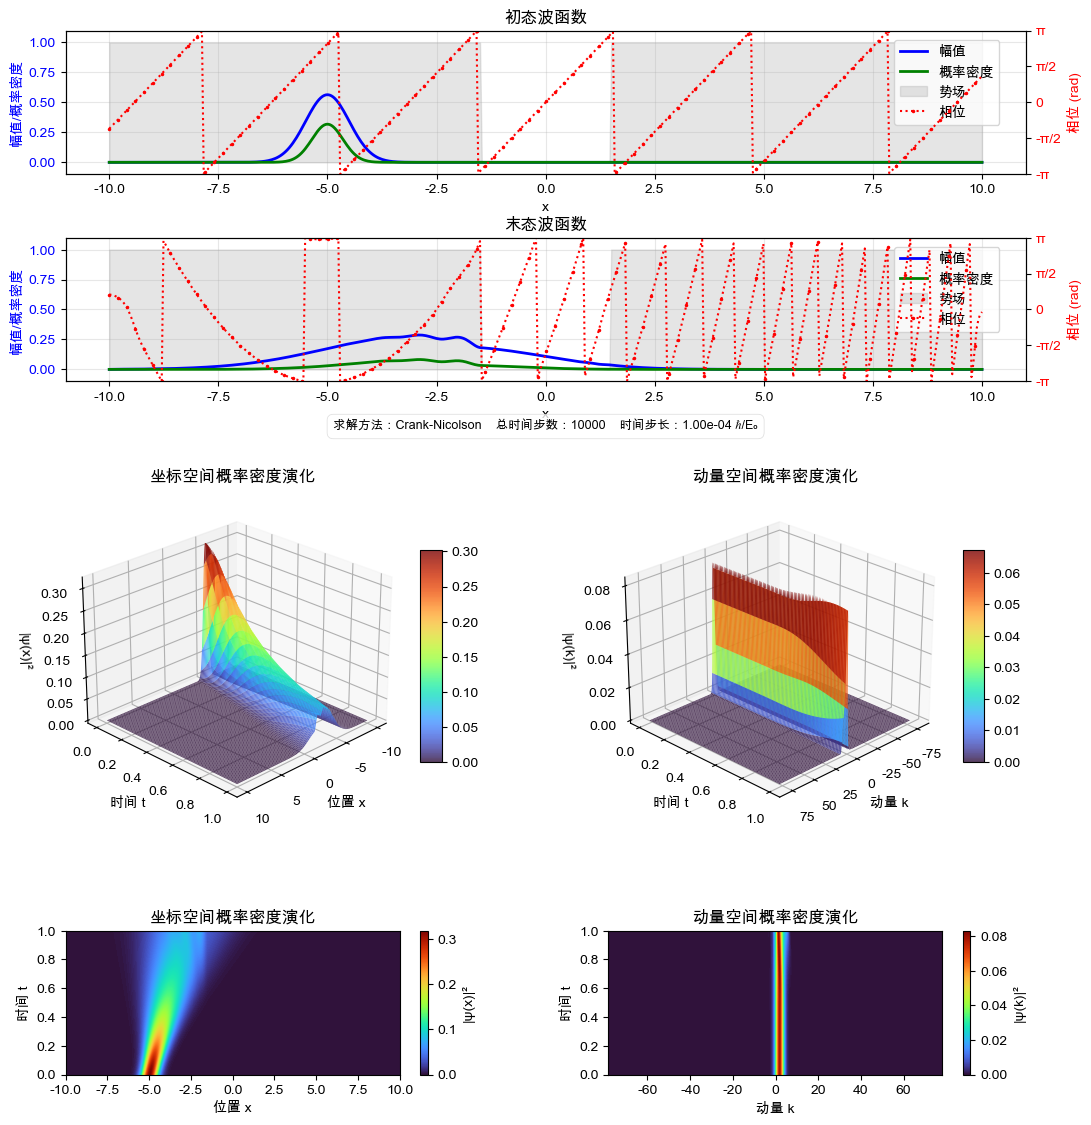
\includegraphics[width=1.0\textwidth]{Problem_2/figs/cn_result.png}
    \caption{Crank–Nicolson解法结果}
\end{figure}

\begin{figure}[H]
    \centering
    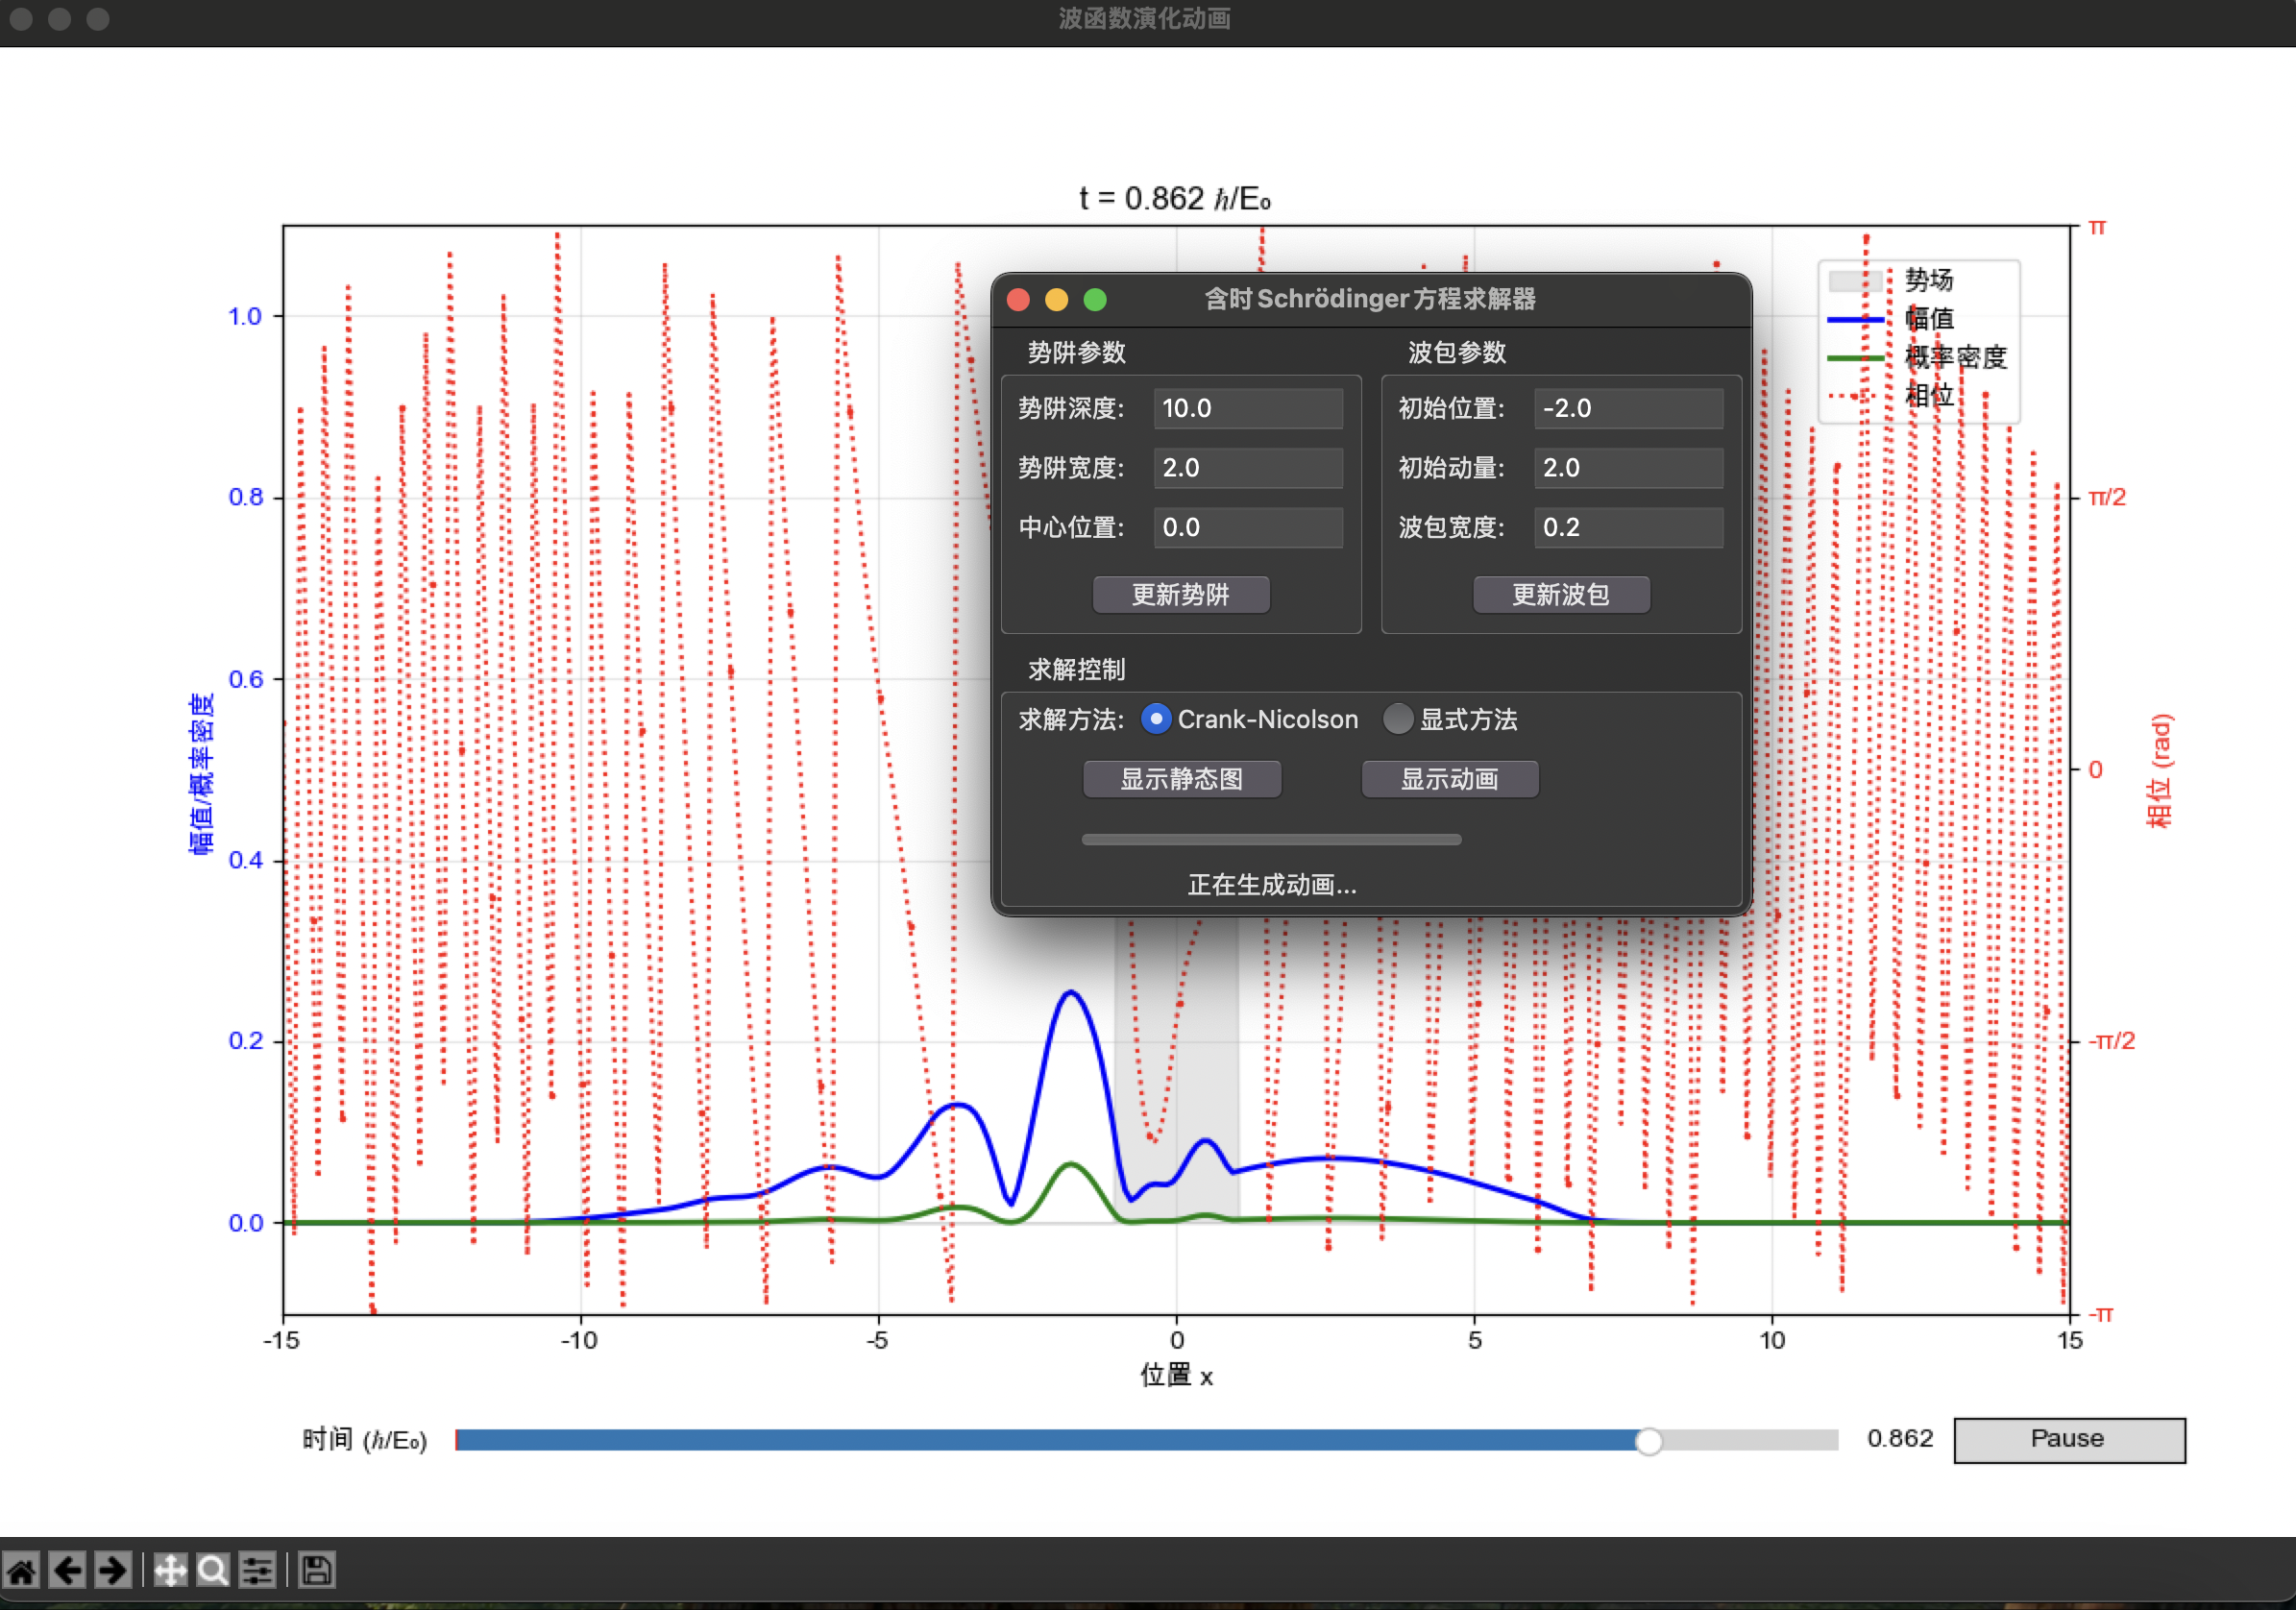
\includegraphics[width=1.0\textwidth]{Problem_2/figs/cn_anim.png}
    \caption{Crank–Nicolson解法中间态(动画截图)}
\end{figure}

\begin{figure}[H]
    \centering
    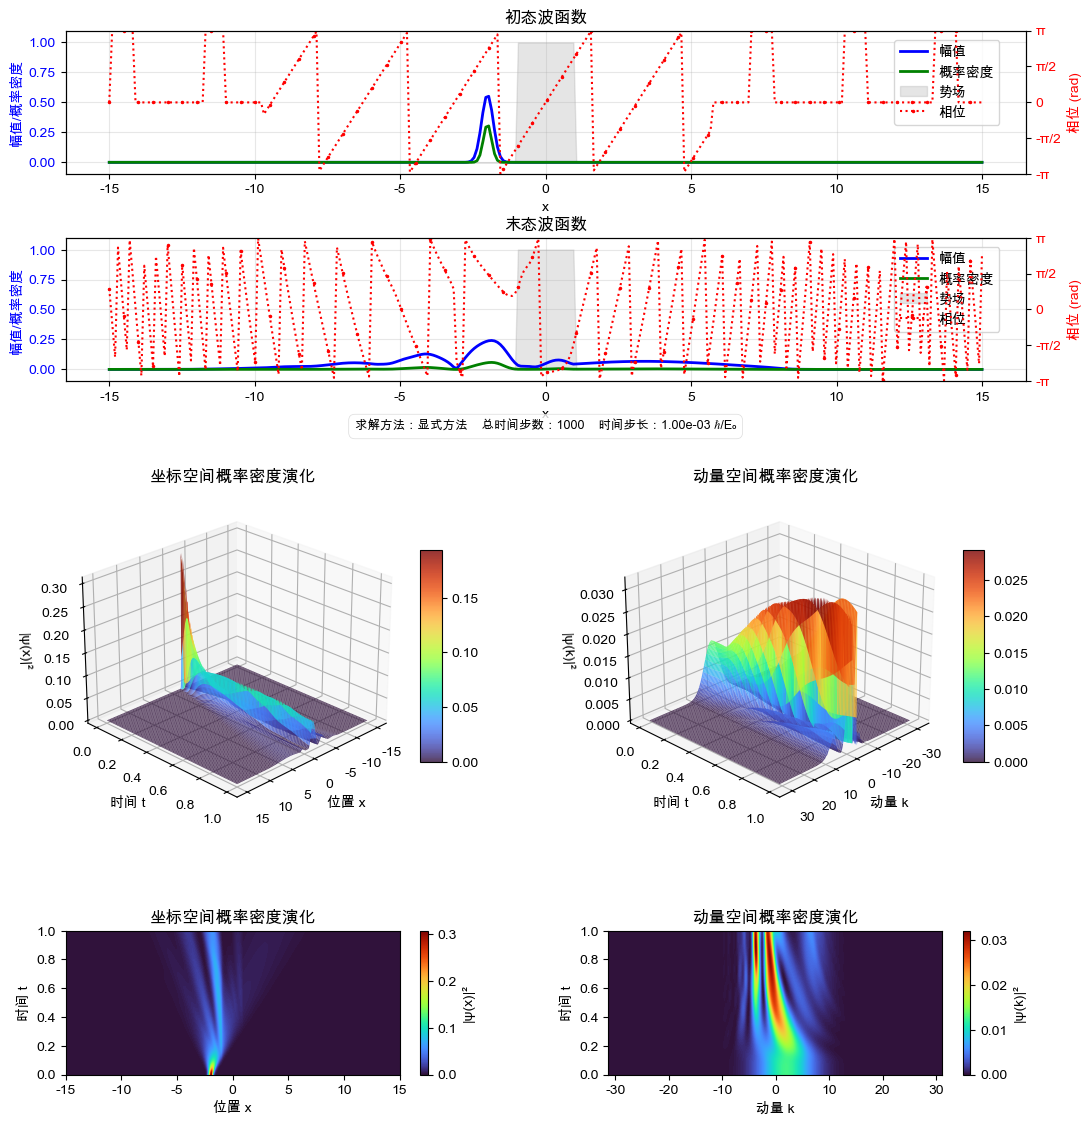
\includegraphics[width=1.0\textwidth]{Problem_2/figs/ex_result.png}
    \caption{显式解法结果}
\end{figure}